\chapter{Evaluation}
\label{ch:evaluation}
In this section, the evaluation of the CASC-SAS approach is discussed.
The goal of the evaluation is to derive quantitative and qualitative characteristics of the approach.
These characteristics are used to verify the applicability of the proposed approach in the presented field of application.
Moreover, the characteristics are used to identify limitations and future work of the proposed approach.
\todo{TODO: Rewrite and add subsections}

\section{Method}
The evaluation is performed theoretically as well as experimentally.
For the theoretical parts of the evaluation, formal and informal methods are used to proof certain characteristics of the proposed approach.
The experimentally performed part of the evaluation is based on the realization presented in \autoref{sec:approach:realization}.

\subsection{Evaluation Areas \& Metrics}
The evaluation aims to derive quantitative and qualitative metrics for different areas of interest.
We propose three areas of interest for the evaluation of the CASC-SAS approach.
The three areas of interest and their corresponding metrics are defined as follows:
\begin{description}
    \item[Security Evaluation] Does CASC-SAS provide security against typical SAS adversaries and attacks?
    \begin{enumerate}
        \item Satisfied security, safety, and availability requirements
        \item Assumed system characteristics
        \item Assumed adversary characteristics
        \item Mitigated attacks
        \item Introduced attack surface
    \end{enumerate}
    \item[Performance Evaluation] Is CASC-SAS capable of securing time-constrained communication of an SAS?
    \begin{enumerate}
        \item Satisfied performance requirements
        \item Assumed communication characteristics
        \item Supported message types
        \item Resistance against network exceptions including congestion, delay, jitter, duplicated packets, lost packets, and out-of-order packet delivery
    \end{enumerate}
    \item[Compatibility Evaluation] Is CASC-SAS a feasible solution for the construction or retrofitting of an SAS?
    \begin{enumerate}
        \item Satisfied compatibility requirements
        \item Assumed device requirements
        \item Additional costs for SAS construction and retrofitting
        \item Feasibility with regard to SAS retrofitting
        \item Cost-benefit efficiency compared to alternative approaches
    \end{enumerate}
\end{description}

\subsection{Testbed}
The component implementations discussed in \autoref{sec:approach:realization} are used to construct a network testbed.
The proposed network testbed is visualized in \autoref{fig:evaluation_test_bed}.
The components depicted in blue represent computers that mimic the behavior of domain-specific senders and receivers of an SAS.
The components depicted in red are part of the CASC-SAS approach.
The components depicted in yellow represent message-forwarding intermediate network devices.

\todo{TODO: Remove simulation from text}
These test environments mimic the behavior of a real interconnected SAS for occurring message exchanges.
The simulation and testbed strategy have differing advantages and disadvantages.
On the one hand, the simulation strategy has the advantage of repeatability and reproducibility due to deterministic behavior, whereas the behavior of the testbed is non-deterministic.
On the other hand, the testbed results are practice-oriented and transferable to the physical SAS domain, whereas the behavior of a real SAS cannot be compared to the deterministic behavior of the network simulation.
\begin{figure}
    \centering
    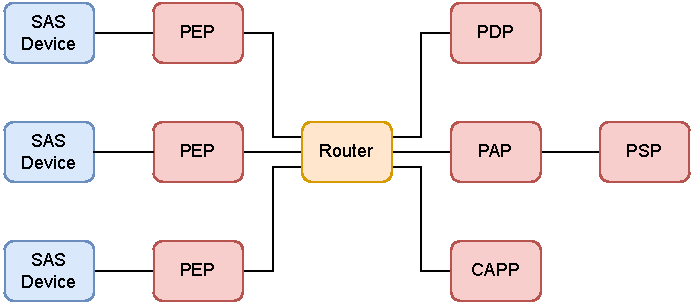
\includegraphics[width=1.0\linewidth]{figures/network_testbed_color.drawio.pdf}
    \caption{Architecture of the network testbed.
    % Architecture of the network testbed used for the experimental evaluation of the CASC-SAS approach. The components depicted in blue represent computers that mimic the behavior of domain-specific senders and receivers of an SAS. The components depicted in red are part of the CASC-SAS approach. The components depicted in yellow represent message-forwarding intermediate network devices.
    }
    \label{fig:evaluation_test_bed}
\end{figure}

\section{Security Analysis}
\todo{TODO: Security analysis for CASA}
\begin{description}
    \item[Definition I.] Unforgeability.\\
    Unforgeability ensures that no adversary can create a valid signature for a message under a policy unless their set of attributes satisfies the policy.
    Formally, unforgeability is defined using a game between a challenger and an adversary:
    \begin{itemize}
        \item Setup: The challenger runs the \texttt{Setup} algorithm to generate the public parameters $PK$ and the master secret key $MSK$. The public parameters are given to the adversary, while the $MSK$ is kept secret.

        \item KeyGen: The adversary can query the \texttt{KeyGen} oracle to obtain private keys for sets of attributes of its choice. The challenger responds with the corresponding private keys.

        \item SignQueries: The adversary can request signatures for messages and policies from the \texttt{Sign} oracle. The oracle returns valid signatures if the queried attributes satisfy the signing policy.

        \item Forgery: The adversary outputs a forged signature $(M^*, T^*, \sigma^*)$ for a message $M^*$ and policy $T^*$. The adversary wins if the following conditions hold:
        \begin{itemize}
            \item The adversary did not request a signature on $(M^*, T^*)$ from the \texttt{Sign} oracle.
            \item The adversary does not possess a private key whose attributes satisfy the policy $T^*$.
            \item The verification algorithm accepts $\sigma^*$ as a valid signature under $T^*$.
        \end{itemize}
    \end{itemize}

    \item[Definition II.] Existential Unforgeability under Chosen-Message Attacks (EU-CMA).\\
    An adversary $\mathcal{A}$ is given access to public parameters, hash oracles, and a signing oracle.
    The scheme is secure if $\mathcal{A}$ cannot forge a valid signature $\sigma^*$ for a new message $M^*$ without knowing the signer's full private key.
    In other words, to create an existential forgery, i.e., output a valid pair of message and signature for a new message, an adversary carrying out a CMA can request valid signatures for any message of his choice \cite{Goldwasser1988}.
    The adversary's advantage in this game is its probability of generating a valid forgery.
    We say the ABS scheme is \textit{existentially unforgeable} if the adversary's advantage is negligible.

    \item[Theorem I.] $\mathcal{S}_{CASA}$ is EU-CMA secure under the Computational Diffie-Hellman (CDH) assumption in the random oracle model.\\
    \textit{Proof.} After querying the signing oracle, assume $\mathcal{A}$ forges a signature $\sigma^*$ for $M^*$ for $ M^*$. The challenger interacts with $\mathcal{A}$ as follows:
    \begin{itemize}
        \item \textit{Setup}: The challenger generates $pk$, $p$, and hash oracles \( H_1, H_2, H_3 \) for \( \mathcal{A} \).
        \item \textit{HashQueries}: The challenger responds to \( H_1, H_2, H_3 \) queries with random values, ensuring consistency.
        \item \textit{SigningQueries}: For $M$ and $\mathsf{Att}_{i}$, the challenger computes:
        \[
        \sigma_i = \big(ppk_{i} \cdot H_3(h)\big)^{x_i},
        \]
        where $h = H_2(M || \mathsf{Att}_{i})$.
        \item \textit{Forgery}: If \( \mathcal{A} \) outputs \( \sigma^* \) for \( M^* \), the challenger extracts \( g^{ab} \) from \( g, g^a, g^b \), solving the CDH problem.
    \end{itemize}
    Thus, $\mathcal{A}$'s advantage is negligible under the CDH assumption. The $\mathcal{S}_{CASA}$ scheme is secure against EU-CMA attacks.

    \item[Definition III.] Collusion Attack.\\
    An adversary $\mathcal{A}$ colludes with the CAPP and corrupted signers to derive private keys or forge valid signatures.
    The scheme is secure if such a collusion does not compromise honest signers and does not allow forgery.

    \item[Theorem II.] $\mathcal{S}_{CASA}$ resists collusion attacks under the Discrete Logarithm Problem (DLP).\\
    \textit{Proof.} Suppose $\mathcal{A}$ colludes with the CAPP to derive $sk_i = (ppk_i, \chi_i)$, then the following steps are performed:
    \begin{itemize}
        \item The CAPP knows $ppk_i = H_1(\mathsf{ID}_i || \mathsf{ATT}_i)^{p}$, but $\chi_i$ is chosen independently by the signer.
        \item The DLP ensures $\mathcal{A}$ cannot derive $\chi_i$ from $y_i = g^{\chi_i}$.
        \item Without $\chi_i$, $\mathcal{A}$ cannot compute:
        \[
        \sigma_i = \big(ppk_i \cdot H_3(h)\big)^{\chi_i}.
        \]
    \end{itemize}
    Thus, collusion cannot compromise security. The $\mathcal{S}_{CASA}$ scheme is secure against collusion attacks.

    \item[Theorem III.] CASC-SAS is resistant against replay attacks.\\
    \todo{Add proof.}
\end{description}

\section{Security Compositions}
\todo{TODO: Security compositions for SABAAC}

\section{Performance Analysis}
\todo{TODO: Security analysis for CASC-SAS}

\section{Compatibility Analysis}
\todo{TODO: Compatibility analysis for CASC-SAS}
Maybe physical compatibility, communication compatibility, economy ("price compatibility")\dots

\section{Discussion}
\todo{TODO: Discussion of results and comparison to different approaches}

\section{Limitations}
\label{sec:approach:limitations}
\todo{TODO: Reactivate reference in approach introduction}
\todo{TODO: Limitations: No intrusion detection but prevention/mitigation, might not be usable for fast messages, not every crypto for every message type, possible new attack vectors by adding new components, applicability to other ics domains, time protocol interference, physical access control -> future work}